% FUNDAMENTAÇÃO

\chapter{FUNDAMENTAÇÃO TEÓRICA}
\label{chap:fundamentacao}
Neste capítulo são apresentados os principais conceitos abordados neste trabalho, sendo estes utilizados como base para a evolução e desenvolvimento do objetivo proposto.

% PROCESSAMENTO DIGITAL DE IMAGENS
\section{PROCESSAMENTO DIGITAL DE IMAGENS}
\label{sec:procimagens}

\par A visão é o principal sentido do ser humano, pois é considerado o sentido mais aguçado e consequentemente avançado desta espécie. Porém a visão dos humanos ainda é limitada, pois podemos ver apenas um espectro de cores\footnote{A visão humana só é capaz de perceber uma faixa do espectro da luz, entre a luz vermelha e violeta, alternando entre o azul, verde e amarelo \cite{Gonzalez2000}.} entre outros limitadores. Isto se diverge de um computador, pois ele é capaz de receber certos ``estímulos'' que o fazem ``ver'' e ``compreender'' imagens além das restrições humanas, como por exemplo o uso de raios X para conceber figuras \cite{Gonzalez2009}.
\par Mas afinal, o que é uma imagem digital? Muitos pensam que esta pode ser definida como um plano cartesiano, por conta de seus \textit{pixels} e da sua estrutura, todavia uma imagem é dita como uma função bidimensional, pois os eixos $x$ e $y$ representam o plano espacial, enquanto $f$ corresponde aos graus de cinza, sendo estes valores considerados finitos. Já os \textit{pixels} (\textit{pels}, \textit{picture elements} ou também \textit{image elements}) são os elementos que compõe a imagem. Cada um destes possuem características diferente, pois ocupam suas posições singulares e possuem valores que podem diferenciar entre si \cite{Gonzalez2009}.

\par O processamento digital de imagens surgiu a partir dos computadores digitais, os quais foram capazes de apresentar uma nova perspectiva de processamento de dados. Este conceito é profundamente discutido e diversos autores discordam entre si, visto que enquanto alguns defendem que o processamento digital de imagens diz respeito a um processo que tem como entrada uma imagem e como saída outra imagem de releitura da primeira, existem autores que discordam e argumentam que tal definição não abrange todo o conteúdo desta área \cite{Gonzalez2009}.
 
\par Portanto, neste trabalho foi considerada a definição de \citeonline{Gonzalez2009}, na qual o autor defende que além da primeira definição apresentada\footnote{Processo que tem como entrada uma imagem e saída outra imagem.}, o processamento digital de imagens engloba procedimentos de compreensão e extração de características para o reconhecimento de determinados objetos.

\subsection{ETAPAS EM PROCESSAMENTO DIGITAL DE IMAGENS}
\label{subsec:etapas}
Segundo \citeonline{Gonzalez2000}, existe uma divisão de 5 etapas para uma rotina em processamento digital de imagens, tais etapas podem ser observadas na \autoref{fig:etapas_processamento_imagens} e correspondem a:
\begin{enumerate}
    \item Aquisição de imagens;
    \item Pré-processamento;
    \item Segmentação;
    \item Representação e descrição;
    \item Reconhecimento e interpretação.
\end{enumerate}

\begin{figure}[!h]
    \centering
    \caption{Passos fundamentais em processamento de imagens digitais.}
    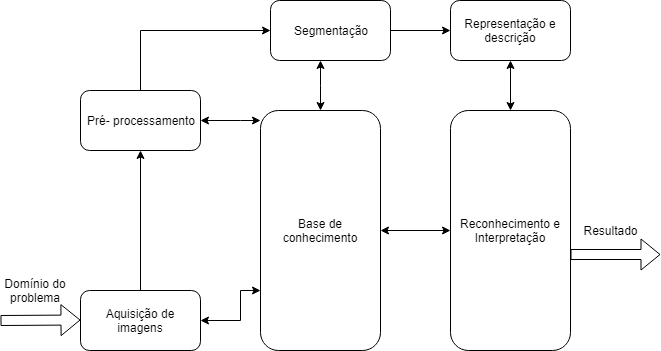
\includegraphics[width=1\textwidth]{./dados/figuras/etapas_processamento_imagens.png}
    \fonte{\citeonline{Gonzalez2000}}
    \label{fig:etapas_processamento_imagens}
\end{figure}

\par Como observado na \autoref{fig:etapas_processamento_imagens}, para a rotina ser executada é necessário um problema que necessite de um resultado final, assim, com as etapas sendo seguidas corretamente o sucesso na tarefa em questão se torna mais provável. 

\par Sendo assim, o processamento digital de imagens inicia-se a partir da aquisição. Para isto, normalmente aparenta-se necessárias câmeras digitais, porém não é apenas tal dispositivo que é capaz de captar sinais e transformá-los em uma imagem digital, também existem outros sensores de imageamento, basta que este possa captar uma banda do espectro de energia eletromagnética. Após a captura é necessário um dispositivo conhecido como digitalizador, o qual é responsável por converter as informações dos sensores que captaram a informação em uma saída digital.

\par A segunda etapa é o pré-processamento de uma imagem que tem como objetivo principal aumentar as chances de sucesso para as próximas etapas, sendo assim necessário aplicar técnicas como as de isolamento de regiões, remoção de ruídos e outras. De tal forma que o resultado final esperado seja de uma imagem consideravelmente melhor quando comparada com a imagem anterior.

\par Em seguida se encontra a considerada mais difícil etapa do processamento digital de imagens: a segmentação. O uso de algoritmos fracos neste momento pode causar uma falha em todo o processo. Apenas algoritmos adequados podem auxiliar e aumentar a garantia de sucesso ao final. Logo, a segmentação é responsável por decompor a imagem em partes ou objetos, obtendo como resultado \textit{pixels}, conhecidos como \textit{raw pixel data}, o que representa uma área e suas bordas, sendo sempre necessária a conversão dos dados para o uso computacional.

\par Já a etapa representação e descrição, também conhecida como seleção de características, é responsável por identificar novas características em uma área anteriormente identificada, as quais são referentes a cor, textura e/ou forma.

\par Por fim, na última etapa, reconhecimento e interpretação, se dá a rotulação de um ``objeto'' previamente segmentado, ou seja, a imagem é totalmente ou parcialmente reconhecida. Além disso, para um conjunto de ``objetos'' é concedido um significado, o que se refere a interpretação \cite{Gonzalez2009}.

%% Para futuras melhorias seria interessante fazer uma nova seção sobre os métodos de descrição de imagem e outro de árvore geradora mínima

% Descrição de imagens
% \section{DESCRIÇÃO DE IMAGENS}
% \label{sec:descimg}



% TEXTURA
\subsection{TEXTURA}
\par A textura, elemento importante neste trabalho, pode ser interpretada por diversas óticas, entre elas a popular, pois é de fácil compreensão já que existem em tudo que é visível. Neste sentido, pode-se entender que não é possível estabelecer uma única definição teórica \cite{liberman1997}. 
\par Para \citeonline{haralickTEXTURA}, texturas podem ser determinadas por seu \textit{``layout''}, organização e níveis de cinza. Entretanto, neste trabalho é adotada principalmente a abordagem de \citeonline{Gonzalez2009}, que reafirmam a impossibilidade de definição formal para a propriedade de textura, mas indicam que a rugosidade, suavidade e outros aspectos seriam resultados de descritores como o algoritmo desenvolvido neste projeto, que descreve e classifica texturas em imagens. 

\begin{comment}
\par As abordagens: estatística, estrutural e espectral são as três abordagens mais utilizadas para descrição de texturas em imagens. \cite{Gonzalez2000}
\par Estatística -> suave, aspera, graunular e etc
\par Estruturais -> tratam de arranjos de primitivas de imagem como a descrição da textura baseada em linhas paralelas regularmente espaçadas.
\par Espectrais -> baseiam-se em propriedades do espectro de Fourier, sendo usadas basicamente na detecção de periodicidade global em uma imagem através da identificação de picos de alta-energia no espectro
\par Falar das abordagens: estatísticas, estruturais e espectrais
\end{comment}
%%%%%%%%%%%%%%%%%%%%%%%%%%%%%%%%%%%%%%%%%%%%%%%%%%%%%%%%%%%%%%%%%%%%

% Arvore geradora mínima
\section{ÁRVORE GERADORA MÍNIMA}
\label{sec:arvore}

\par Árvores geradoras mínimas costumam solucionar diversos problemas, um exemplo de sua performance está em projetos de circuitos eletrônicos, pois muitas vezes é necessário fazer a conexão entre pinos de modo que estes estejam eletricamente equivalentes. Tal conexão deve ser feita utilizando o menor custo possível, ou seja, o mínimo de material (fiação), isto caracteriza um problema que procura encontrar a MST dado um grafo \cite{algoritmos}.

\par Considerando um grafo conexo não dirigido $G$ que pode ser representado por $G = (V, E)$, onde $V$ é o conjunto de todos os vértices e $E$ o conjunto de todas as ligações possíveis entre os vértices do grafo $G$. Todas as arestas formadas por uma conexão de um vértice ao outro, representado por $(u, v) \in E$, devem possuir pesos, ou seja, o custo de um vértice ao outro, que simboliza $w(u, v)$. O que é procurado é uma conexão que esteja contida em $E$ de forma que gere um novo grafo $T$ acíclico e conecte todos os vértices. Dessa maneira, conclui-se que uma árvore geradora mínima é um grafo acíclico que busca percorrer o menor caminho possível e que está contido e gerado a partir de um outro grafo \cite{algoritmos}.

\par Uma representação de um grafo conexo e uma árvore geradora mínima pode ser observada na \autoref{fig:mst}. Todas as arestas pertencem ao grafo, sendo as arestas sombreadas\footnote{Como a aresta que liga os vértices $a$ e $b$} correspondentes à árvore geradora mínima. Também é possível observar que todas as arestas são ponderadas e que o peso total da árvore corresponde a 37. Além disso, esta não é a única MST presente no grafo, pois caso a aresta $(a, b)$ seja trocada pela aresta $(a, h)$, haverá outra MST também com o peso total 37 \cite{algoritmos}.

\begin{figure}[!h]
    \centering
    \caption{Grafo conexo e MST}
    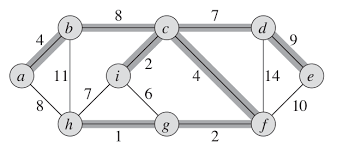
\includegraphics[width=0.7\textwidth]{./dados/figuras/grafo-mst.png}
    \fonte{\citeonline{algoritmos}}
    \label{fig:mst}
\end{figure}

\par O termo conhecido como ``árvore geradora mínima`` é uma redução da sentença ``árvore geradora de peso mínimo``. Tal explicação se faz necessária, pois existe a possibilidade de que o termo mais comum gera a má interpretação de que o número de arestas de uma árvore geradora foi diminuído, o que não corresponde à verdade.

\subsection{ALGORITMOS}
\label{subsec:algoritmosmst}

\par Existem dois algoritmos principais que buscam resolver o problema da MST, estes são: o algoritmo de Kruskal e o algoritmo de Prim. Ambos são considerados gulosos\footnote{Segundo \citeonline{algoritmos}, os algoritmos gulosos consideram sempre a escolha do momento como a melhor escolha possível, acreditando que esta traga consigo o melhor resultado.}. Apesar de não garantirem resultados considerados excelentes, isto se diverge, ou seja, os algoritmos gulosos podem produzir uma MST dado um determinado grafo.
\par Neste projeto, será utilizado o algoritmo de Prim, pois segundo \citeonline{igraph}, este é implementado na biblioteca \textit{igraph} para o método que gera uma MST, dado um grafo e seus pesos. Maiores detalhes, sobre esta e outras bibliotecas utilizadas podem ser observados na \autoref{sec:tecnologiasferramentas}.

% Uso de Grafos em descrição de imagens
\section{USO DE GRAFOS EM DESCRIÇÃO DE IMAGENS}
\label{sec:usografosdescimg}

\par A partir de pesquisas sobre o estado da arte desta área foi possível concluir que, no momento atual de desenvolvimento deste trabalho, não existem publicações sobre a aplicação de MST para a descrição de texturas em imagens, sendo os únicos encontrados, trabalhos que utilizam árvores geradoras mínimas para a segmentação, registro, detecção de imagens ou outros.

\par Sendo assim, apesar de poucos trabalhos buscarem a utilização de outros tipos de algoritmos com grafos e árvores para descrição de imagens, é possível observar que nestes há uma melhoria considerável, o que estimula o desenvolvimento de novos métodos de pesquisa em vários campos de processamento de imagens e computação visual, assim como proposto por este trabalho.

\subsection{\textit{SHORTEST PATHS} EM DESCRIÇÃO DE IMAGENS}
\label{subsec:trabalho-jarbas}

\par O estudo que mais se assemelha com a proposta deste trabalho é o de \citeonline{jarbas-color-texture}, que tem como título: \textit{Color Texture Classification Using Shortest Paths in Graphs}. Apesar de utilizarem o algoritmo de \textit{shortest paths}, caminho mais curto, se aproximam pelo estudo de textura da imagem, a ligação entre os vértices e a forma como a imagem é ``tranformada'' em grafo.

\par Neste trabalho, o algoritmo desenvolvido obteve resultados significativos e potentes na extração de informações presentes na textura das imagens analisadas, sobressaindo até mesmo algoritmos bem estabelecidos atualmente. Desta forma, pode-se concluir que a utilização de grafos para descrição de texturas em imagens se mostra como uma boa oportunidade de campo novo a ser explorado que pode auxiliar no aumento da acurácia e confiança em sistemas de computação visual.
